\documentclass[a4paper,11pt]{report}
\usepackage[T1]{fontenc}
\usepackage[english,ngerman]{babel}
\usepackage[utf8]{inputenc}
\usepackage{titlesec}
\usepackage[onehalfspacing]{setspace}
\usepackage[autostyle=true]{csquotes}
\usepackage{geometry}
\usepackage{fancyhdr}
\usepackage[
  backend=bibtex,
  style=authoryear,
  firstinits=true,
  uniquename=init,
  sortlocale=de_DE
]
{biblatex}
\usepackage{graphicx}
\graphicspath{ {./appendix/} }
\DeclareNameAlias{sortname}{last-first}
\DeclareFieldFormat*{title}{#1}
\DefineBibliographyStrings{ngerman}{
   andothers = {{et\,al\adddot}},            
}
\addbibresource{ref.bib}
\geometry{
  left=25mm,
  right=35mm,
  top=30mm,
  bottom=20mm,
  bindingoffset=5mm
}
\titleformat{\chapter}[display]
  {\normalfont\bfseries}{}{0pt}{\Large}
\titlespacing{\chapter}{0pt}{25pt}{10pt}

\renewcommand{\rmdefault}{phv} % Arial
\renewcommand{\sfdefault}{phv} % Arial
\renewcommand{\headrulewidth}{0.1pt} 
\interfootnotelinepenalty=10000

\usepackage{etoolbox}
\makeatletter
\patchcmd{\chapter}{\if@openright\cleardoublepage\else\clearpage\fi}{}{}{}
\makeatother

\begin{document}
\title{Wurden die richtigen Lehren aus der
    Finanzkrise 2007-2009 gezogen?}
\author{%
    Facharbeit im Leistungskurs Sozialwissenschaften \\
    Ravensberger-Gymnasium Herford \\ \\
    \textit{eingereicht bei} \\
    Herrn Visser \\ \\
    \textit{vorgelegt von} \\
    Gabriel de Souza Tomitsuka 
    }
\date{Herford, Oktober 2019}
\maketitle
\tableofcontents
\newpage
\chapter{Einleitung}
\section{Themawahl}
Laut dem Gesch\"aftsf\"uhrer der Investmentbank J.P. Morgan
Chase Jamie Dimon war die Woche des 15. Oktober 2008, also ab dem
Tag, wo Lehman Brothers Insolvenz angemeldet hat,
mit der Woche des \enquote{Great Crashes} ab dem 24. Oktobers 1929
von einer finanzwirtschaftlichen Perspektive vergleichbar,
allerdings hat die rechtzeitige Reaktion der Regierungen und
Regulatoren das Schlimmste vermieden \parencite{dimonyt}.

Ich habe mich oft gefragt, wie ein Markt, der
von kleinen, amerikanischen Regionalbanken mit
staatlicher Unterstützung
dominiert wird, zum Fall von als \enquote{Too Big To
Fail} verstandene Investmentbanken wie Lehman
Brothers und Merill Lynch
führen konnte. Besonders interessant fand ich,
dass auch Banken in anderen Kontinenten (wie
bspw. die Dresdner Bank) dadurch
aufgekauft werden mussten.

Ich wollte genauer
ermitteln, wie stark diese Vernetzung damals
war und heute ist, und ob
die kurzfristigen Maßnahmen durch
Zentralbanker, Banken/Fonds und Regulatoren
womöglich eine noch schlimmere Krise
vermieden haben -- also ob die Behauptung Dimons
stimmt.

Allerdings werde ich mich nicht besonders
lange mit einer historischen Betrachtung
beschäftigen, ob die kurzfristigen
Maßnahmen wie geplant wirkten, sondern viel
mehr mit der Fragestellung, ob die mittel- und
langfristigen Maßnahmen die Welt
auf die nächste Rezession richtig vorbereitet
haben --- alle Händler und Investmentbanker, mit
denen ich mich im Rahmen meiner Facharbeit ausgetauscht habe, waren
der Ansicht, dass wir uns spät im Marktzyklus
befinden, und die Frühindikatoren zeigen
ähnliche Signale.

Daher ist es besonders wichtig zu
überprüfen, inwiefern das gesamtwirtschaftliche System auf die nächste Rezession vorbereitet ist.
\section{Vorgang}
Die Ursachen für die Finanzkrise 2008 können 
in zwei Gruppen unterteilt werden: Ursachen der Immobilienkrise
in den Vereinigten Staaten und die finanzwirtschaftliche
Ursachen der globalen Finanzkrise.

\"Uber die realwirtschaftlichen Ursachen besteht weithin
Einigkeit innerhalb der Wirtschaftswissenschaften, daher
werde ich verk\"urzt auf sie eingehen.

Um die finanzwirtschaftliche Ursachen zu erläutern, werde
ich erst auf die theoretische Grundlage des Finanzsystems
nach den Deregulierungen in den 1970er Jahren eingehen,
sowie die der Bankentheorie. Daraufhin werde ich die 
Instrumente untersuchen, die dazu beigetragen haben,
dass diese theoretische Grundlage nicht mehr galt --- 
dazu geh\"oren Asset-Backed Securities (ABS),
Collateralized Debt Obligations (CDO) und
Credit Default Swaps (CDS). Daraufhin werde
ich untersuchen, wie genau sie für die
Krise mitverantwortlich sind. Ferner werde ich
die Frage erörtern, ob es andere Instrumente
oder Anlageklassen gibt, die eine
besondere Wirkung auf die Krise hatten, die in
der Öffentlichkeit nicht angekommen ist.

Daraufhin werde ich die kurzfristige Reaktion
der Regulatoren und Zentralbanker ab 2008
untersuchen. Genauer werde ich auf
Sofortmaßnahmen wie die kontroverse
Bankenrettung, (bis heute anhaltende)
Zinssenkungen, <etc> eingehen.
Schließlich werde ich auf die mittel- und
langfristigen Maßnahmen, inkl. Basel
III und CRD eingehen.

Schließlich werde ich mit Bezug auf
privaten Gesprächen mit Händlern,
Risikoverwaltern und Investmentbankern 
sowie \"offentliche Interviews mit F\"uhrungskr\"aften
aus dem Finanzsektor bzw.
Ver\"offentlichungen finanzieller Institutionen
erörtern, ob die Maßnahmen die europäische
Wirtschaft ausreichend auf die
Herausforderungen der Zukunft vorbereiten.

\chapter{Amerikanische Immobilienkrise}
Über die realwirtschaftliche Ursachen der Krise besteht
weithin Einigkeit in den Wirtschaftswissenschaften: 
der Kreditboom in den USA und die Immobilienblase.
Im Folgenden werde ich erläutern, wie diese entstanden
sind und wie sie zur Krise beigetragen haben.

\section{Der Hypothekenmarkt}
Aus den f\"unfundsiebzig Millionen H\"ausern im
Privateigentum 2007 in den USA, wurden auf etwa f\"unfzig Millionen
Hypotheken aufgenommen (Buffett, 2018).
In der Zeit zwischen 2002 und 2007 hat sich das
Schulden zu Nationaleinkommen-Verhältnis
der USA von 3,75:1 auf 4,75:1 erhöht.
Um die letzte Erhöhung der Schulden in
dieser Größenordnung zu erreichen, hat man davor
das gesamte Jahrzehnt der 1990er
gebraucht \parencite[S. 195f.]{acharyar}.

Durch das Schaubild in Appendix 1 wird deutlich,
dass der Wachstum der Immobilienpreise keine Verbindung
mit den finanziellen Zugewinnen der Amerikaner hatte,
und zumeist spekulativ war. 

Laut dem US-amerikanischen
Großinvestor Warren Buffett war die Einstellung
des durchschnittlichen amerikanischen
B\"urgers zu der Zeit,
dass die Immobilienpreise ewig weitersteigen w\"urden,
und basierend auf dieser Erwartung durch das Haus
gesicherte Kredite aufgenommen haben (Buffett, 2018).

\subsection{Der Subprime-Markt}
Viele Immobilienkredite wurden von Menschen, die selbst
in einer Niedrigzinsumgebung sich die Immobilie nicht leisten
konnten, die sie erworben haben.
Dazu kommen die strategischen Anreize, um Kreditnehmer
mit wenig Bonit\"at (Subprime) zu erwerben. Dazu z\"ahlen
Kredite ohne Einkommensbeweise (siehe Appendix II), 
und hybride Kredite mit Teaserraten. Sie wurden in "2/28\"\-- oder
"3/27\"\--Modellen verkauft, die sehr attraktive, fixe Zinsraten
f\"ur die ersten zwei bzw. drei Jahre hatten, und
f\"ur die letzten achtundzwanzig bzw.
siebenundzwanzig exorbitant hohe Zinss\"atze\footnote{
  wie solche Kredite m\"oglich waren, wird in 3.3 erl\"aurtert}.
Diese waren so konstruiert, dass sie in ausgesprochen vielen
F\"allen den Kreditnehmer zur Insolvenz f\"uhrten --
nach diesen wenigen Jahren hatte ein Subprime--Kreditnehmer
keine Wahl. Entweder stiegen die Immobilienpreise deutlich
und er kann die Immobilie neu finanzieren, oder er muss
Insolvenz erkl\"aren \parencite[S. 208]{acharyar}.

Unter diesen Umst\"anden wird deutlich, dass diese eine
Umgebung war, wo selbst eine verringterte Wachstumsrate
der Immobilienpreise ausgereicht h\"atte,
um den Binnenmarkt in den USA zu schaden -- wenn sich
Menschen darauf verlassen, dass Immobilienpreise
steigen m\"ussen, damit sie ihr Haus \"uberhaupt behalten
d\"urfen, ist ein Sturz mit dramatischen Folgen verbunden.

\section{R\"uckgang ab 2006}
Allerdings passierte ab November 2006 genau das.
Das Wachstum des realen HPI (House Price Index,
Purchase Only) wurde Anfang 2006 langsamer, und
ab November 2006 sank es (Appendix 3).

In August 2006 ist der Anteil der insolventen
Immobilien, die an Subprime Kreditnehmer verkauft wurden,
auf 7.74\% gestiegen (vgl. August 2005: 5,53\%).

Kurz daraufhin waren die ersten spezialisierte
Kreditgeber im Bereich Subprime ebenfalls insolvent - 
Ownit Mortgage Solutions Inc. hat Dezember 2006 Chapter 11
Bankruptcy Protection\footnote{Demnach kann eine insolvente
Firma eine Sanierung bzw. Reorganisation vorschlagen,
um ihre Kredite versp\"atet zahlen zu k\"onnen, und somit
das Gesch\"aft zu retten. In Ownits Fall war dieser Plan nicht
erfolgreich.} beantragt. Ownit war der elftgrößte Kreditgeber
im Subprime-Sektor \parencite{wsjdoss}. 

Am 12. M\"arz 2007 hat der zweitgr\"oßte Kreditgeber im Bereich
Subprime, New Century Financial Corporation, aufgeh\"ort, neue
Kredite zu geben. Sie meldeten Insolvenz einen Monat sp\"ater
an\footnote{Die Insolvenz hatte unterschiedliche Gr\"unde -
zus\"atzlich hat New Century keine Investoren mehr gefunden
und sie haben mehrere Sammelklagen verloren.}. 2007 haben sie noch
etwa 60 Milliarden Dollar an Krediten vergeben \parencite{nytcres}.

Subprime-Kreditnehmer, die hybride Kredite in "2/28\"\-- oder
"3/27\"\--Modellen gekauft haben, wollten zu dieser Zeit ihre Kredite neu finanzieren.
Allerdings war dies nicht m\"oglich, da eine Refinanzierung nach
Wertverlust der Immobilie keinen Sinn ergibt. Dies  f\"uhrte zu
einer Welle von Insolvenzen, die fast zwangsl\"aufig sonstige
Wirkungen auf den US-Binnenmarkt haben w\"urde.
Die durchschnittliche amerikanische Familie, dessen Haus
hypothekarisch belastet war und dessen Haus etwa 35\% ihres
Gesamtverm\"ogens betrug, hat 2008 aus diesen Gr\"unden deutlich weniger
konsumiert als in den Vorjahren -- eine Rezession war zu erwarten. 
\parencite[196]{acharyar}

\chapter{Globale Finanzkrise}
Warum diese Faktoren aber zu einer Finanzkrise gef\"uhrt haben,
durch die viele der gr\"oßten Finanzinstitutionen
der Welt gefallen sind und Kapitalm\"arkte eingefroren haben,
ist allerdings viel weniger klar. Um die am weitesten verbreitete
Theorie zu erkl\"aren, ist notwendig, zu verstehen, warum das
System versagt hat. Daf\"ur werde ich erst die alte Finanzordnung vor 
den 1980ern erkl\"aren, um daraufhin 

\section{Die alte Finanzarchitektur}
Nach der Weltwirtschaftskrise 1929 war die mehrheitliche politische
Meinung, dass unregulierte
Finanzm\"arkte intrinisisch instabil sein und stark reguliert
werden m\"ussen, um schwere wirtschaftliche Krisen und politische bzw. gesellschaftliche
Unruhe zu vermeiden. \parencite[S. 563f.]{crottycam}.

Das Bretton-Woods-System,
entwickelt nach den Vorstellungen von John Maynard Keynes,
Hyman Minsky und Harry Dexter White, hat eine neue globale W\"ahrungs-
und Handelsordnung in Kraft gesetzt, welche Regierungseingriffe
in W\"ahrungs- und Finanzkrisen erleichtert, und sollten es
vereinfachen, dass Regierungen Maßnamen (wie z.B. gegen die Arbeitslosigkeit) ergreifen
k\"onnen, ohne sich Sorgen um ihre Zahlungsf\"ahigkeit machen zu m\"ussen.

Durch die IMF und die Weltbank sollten Liquidit\"atsprobleme
vermieden werden und Regierungen und Regulatoren langfristig handlungsf\"ahiger werden
\parencite[S. 31f.]{bordo}.

\section{Die neue Finanzarchitektur}
Wirtschaftliche Turbulenzen in den 1970er Jahren f\"uhrten
zu einen Paradigmenwechsel: die \"Uberzeugung, dass staatliche
Vorschriften im Finanzsektor mehr Schaden als Nutzen anrichten.
\"Uber die Zeit ersetzte die neoklassische Theorie den 
Keynesianismus und die enge regulatorische Umgebung wurde gelockert
-- Geschäftsbanken sollten wenig reguliert werden, Investmentbanken
noch weniger und Schattenbanken (bspw. Hedge- und Private-Equity-Fonds) kaum.

Die Maßnahmen der Deregulierung in den USA fingen in 1980 an. Der
\textit{Depository Institutions Deregulation and Monetary Control Act (DIDMCA)}
entfernte die Zinsobergrenze und erteilte Banken und anderen
finanziellen Institutionen die Erlaubnis, Darlehen mit variablen
 Zinsen zu vergeben\footnote{Wegen DIDMCA k\"onnen bis heute
 Institutionen, die Kurzzeitkredite an Subprime-Kreditnehmer
 vergeben, Zinss\"atze bis 700\% im Jahr zu verlangen.}
\parencite[6--8]{sherman2009short}.

Zwar hat DIDMCA die Dynamik des Kreditmarktes in Amerika nachhaltig
ver\"andert, allerdings war die einflussreichste Deregulierungsmaßname
die Lockerung und anschließende Aufhebung des
\textit{Glass-Steagall Act of 1933}.
Die gesetzliche Trennung zwischen Geschäfts- und Investment-Banken
beabsichtigte eine Vermeidung von Interessenkonflikten und 
\"uberm\"aßiger Risikobereitschaft durch Geschäftsbanken.
In der Praxis bedeutete das, dass eine Gesch\"aftsbank keine 
Verbriefungen b\"urgen oder verkaufen konnte und ausschließlich
erstklassige Wertpapiere f\"ur sich kaufen konnte.

In 1986 hat die \textit{Federal Reserve} Glass-Steagall neu interpretiert:
Geschäftsbanken durften bis zu 5\% ihres Umsatzen durch Investmentbanking
erzeugen.

In 1996 ist die \textit{Federal Reserve} einen Schritt weiter gegangen:
Bankholdinggesellschaften durften bis zu 25\% ihres Umsatzes durch
Investmentbanking generieren, was Glass-Steagall in der Praxis aufhebt,
da nahezu alle Institutionen unter der 25\%-Grenze bleiben k\"onnten.
In 1999 hat die Clinton-Regierung Glass-Steagall offiziell aufgehoben.

Ein weiterer Schritt war die \textit{
  Riegle-Neal  Interstate  Banking  and  Branching Efficiency Act}, die
die Restriktionen des Bankings \"uber die Grenzen eines US-Bundesstaats
entfernt hat. Durch Fusionen sank die Zahl der amerikanischen 
Banken um 27\% zwischen 1990 und 1998 \parencite[8--12]{sherman2009short}.

\subsection{Strukturelle Probleme}
Der postkeynesische \"Okonom James Crotty behauptet, die neue Finanzstruktur
habe auch in der Theorie Probleme. Ein Hauptargument der Neoklassik sei, dass
Kapitalm\"arkte Wertpapiere richtig bepreisen und das Risiko gut einsch\"atzen
k\"onnen. Marktteilnehmer seien dementsprechend in der Lage,
richtige Entscheidungen entsprechend ihres Risikoprofils zu treffen.
Somit seien Finanzkrisen sehr unwahrscheinlich, da Marktteilnehmer nur so viel
Risiko aufnehmen w\"urden, wie sie tragen k\"onnen. Allerdings soll dieses Argument
keine empirische Beweise haben und auf unrealistische Annahmen basiert sein 
\parencite[563--565]{crottycam}.

\section{Grundlage des modernen Bankings}
Die klassische Theorie des Bankings ist, dass Banken als Vermittler
zwischen Einleger und Kreditnehmer agieren. Kreditgeber legen ihr Geld
in die Bank ein und kriegen daf\"ur Zinsen, w\"ahrend die Banken die
Bonit\"at der m\"oglichen Kreditnehmer evaluieren und dementsprechend
Entscheidungen treffen, wem sie Geld leihen.

Dadurch, dass das Geld der Kreditgeber angelegt wird, kann nicht jeder
Kreditgeber sein Geld zum gleichen Zeitpunkt zur\"uckfordern, obwohl er
in den meisten F\"allen einen Anspruch darauf hat -- Um dieses Risiko
zu vermeiden, werden Einlagen bis zu einem bestimmten Niveau durch
die Regierung gesichert (in den USA 100 Tausend Dollar, in der EU 100 Tausend Euro).

Im Gegenzug erwarten Regierungen, dass Banken bestimmte Kapitalpuffer
bereithalten. Zu dem Zeitpunkt der Krise war das mindestens 8 Prozent\footnote{
  Diese Zahl wird durch die Bank für Internationalen Zahlungsausgleich
  festgelegt. Mitglieder sind nahezu alle Industrienationen und viele
  weitere Entwicklungsl\"ander.
} des Kapitals der Bank. \parencite[197--198]{acharyar}

Allerdings ist es aus Bankenperspektive unglaublich teuer, so viel
Kapital als Puffer zu halten. Es gibt aber einen Ausweg.

\subsection{Verbriefungen}
Im amerikanische Bankensystem waren im Jahre 2008 etwa 7 Billionen US-Dollar
in Einlagen und etwa 14 Billionen US-Dollar an Krediten\footnote{
  Davon waren \$1,3 Billionen Subprime-Hypotheken, \$3,3 Billionen kommerzielle
  Hypotheken und \$5.8 Billionen Prime-Hypotheken.}.
Der Grund f\"ur diese Diskrepanz sind Verbriefungen --
durch sie werden Banken nicht mehr nur Vermittler
zwischen Einleger und Kreditnehmer, sondern zwischen
\textit{Investoren} und Kreditnehmer.

Im Gegensatz zu Anlegern brauchen Investoren klare
Zahlungsstr\"ome und m\"ussen wissen, wo und wie 
ihr Geld investiert wird. Außerdem m\"ussen
das genaue Risiko einzustufen -- diese Rolle
wurde den Ratingagenturen wie Fitch Ratings, Moody's und S\&P
abgegeben.

\textit{Mortgage-Backed Securities (MBS)} sind die
\"altesten und am gr\"oßten bis heute eingesetzte
Verbriefungen. Sie bestehen aus den Geldfl\"ussen
von Zins- und Tilgungszahlungen
mehreren Tausenden Hypotheken. Sie sind mit zwei
Risiken verbunden: eine Fr\"uhtilgung
oder die Insolvenz des Kreditnehmers. 
Amerikanische Immobilien waren mehrheitlich verbrieft --
etwa 55\% der Immobilienkredite waren .


In diesem Rahmen sind die Geb\"uhren, die Banken
durch Verbriefungen verdienen, zu einer
Haupteinnahmequelle der Banken geworden. Da eine
Bank duch das Veraufen einer Verbriefung
das Risiko an eine andere Person oder Institution
\"ubertr\"agt, braucht sie keine Kapitalpuffer.

Ein Vorteil des System der Verbriefungen
ist, dass wenn fehlerfrei angewandt, es Risiko
so aufteilt, dass Risiko nicht auf eine Institution
konzentriert ist, sondern immer auf vielen Marktteilnehmern,
die nur so viel Risiko aufnehmen, wie sie tragen k\"onnen.
Das reduziert das allgemeine systematische Risiko \parencite[198--201]{acharyar}.
Allerdings gibt es auch große Probleme.

\subsection{Falsche Anreize}
Durch die \"Ubertragung des Risikos werden
viele falsche Anreize f\"ur Vermittler geschaffen. 
Das l\"asst sich leicht am Beispiel der Subprime-Hypotheken merken.
Wie in Abbildung 2 ersichtlich (siehe Appendix), haben viele
Hypothekenspezialisten und -banken keinen Grund gehabt, die 
Bonit\"at ihrer Kunden zu \"uberprufen, da sie die Hypotheken
an eine große Bank unabh\"angig davon verkaufen k\"onnten
und ihre Kommission verdienen w\"urden, egal was den 
Immobilien passiert \parencite[565]{crottycam}.

Die großen Investmentbanken haben ebenfalls falsche Anreize geschaffen.
Die Formel zur Bildung der Bonussen hat ausschließlich auf die sofortigen
Gewinne bzw. Verluste durch die Bildung und den Verkauf der Verbriefungen.
Die mittel- und langfristigen Folgen ihrer Entscheidungen war hierbei irrelevant.
Merill Lynch, die Investmentbank die im Rahmen der Finanzkrise von
Bank of America aufgekauft werden musste, um am Leben zu bleiben,
dient hier als gutes Beispiel. Sie haben 2008 \$3.6 an Bonussen ausgesch\"uttet,
obwohl die Bank \$27 Milliarden verloren hat (genug, um fast zehn Jahre an Profiten
\enquote{auszugleichen}) \parencite[565]{crottycam}.

Kreditratingagenturen haben eine große Rolle gespielt, da zum einen
die Größe der Kapitalpuffer
von dem Rating der Anlagen abh\"angig ist, und Banken
oft aus verschiedenen Gr\"unden ihre eigenen Verbriefungen
gekauft haben. Dadurch, dass die Kredite in Triple-A-Wertpapiere
verpackt waren, mussten Baken deutlich weniger Kapitalpuffer halten
 -- im System nach Basel II brauchte ein Triple-A-Wertpapier
 nur die H\"alfte des Kapitalpuffers eines klassischen Kredits.

Investmentbanken haben die Tatsache ausgenutzt,
dass sie frei w\"ahlen durften, welche Agentur f\"ur die
Ratings ihrer Kreditprodukte verantwortlich ist. Wenn die Ratings
einer Agentur schlechter als gehofft waren, haben sie Agenturen
gewechselt.

Dadurch erm\"oglichten Kreditratingagenturen
den Verkauf an Institutionen wie Geldmarktfonds,
die gesetzlich dazu
verpflichtet sind, haupts\"achlich in die sichersten Wertpapiere
zu investieren. Da diese Fonds grunds\"atzlich
wenige sehr rentable M\"oglichkeiten haben,
waren f\"ur sie indirekte Investitionen in 
MBS und CDOs besonders attraktiv. Diese geschahen \"uber
\textit{Asset-Backed Commercial Paper} (ABCP), die oft ignoriert werden.

Diese waren f\"ur Banken sehr risikoreich,
da Geldmarktfonds nur kurzfristig
geliehen haben -- Banken mussten regelm\"aßig ihre Schulden erneuern.
Sie haben also kurzfristig geliehenes Kapital, das jederzeit verschwinden
konnte, verwendet, um illiquide Wertpapiere, die langfristig gehalten wurden,
zu finanzieren \parencite[201]{acharyar}.

Banken haben diese Strategie verwendet um Verbriefungskommissionen
zu erh\"ohen, und das war in den Boomjahren extrem profitabel.
Als sich die Lage auf dem Subprime-Kreditmarkt aber verschlechtert hat,
haben sich diese Fonds entschieden, ihre Kredite nicht zu erneuern.
Da Investmentbanken die Wertpapiere in den ABCPs garantiert haben, mussten
sie diese nun auf ihre eigene Bilanz zur\"uckbringen. Ungef\"ahr \$400 Milliarden
an Verbriefungen haben dadurch im Jahre 2008 die Bilanzen globaler Banken
erreicht \parencite[570]{crottycam}.

Im Interview mit mir erkl\"arte T. Rossi, dass dieser Aspekt
zum Fall von Lehman Brothers und Merill Lynch gef\"uhrt hat.
Diese Banken haben vom einen Tag auf den n\"achsten Hunderte
Milliarden mehr an Verbindlichkeiten gehabt, ohne einen Cent
Kapital daf\"ur zu haben.
Dadurch mussten Banken in wenigen Monaten
mehr Kapital auftreiben, als ihre Bank wert ist (siehe Appendix: Interview 3).
Kaum Investoren waren \"uberhaupt in der Lage,
die ben\"otigte Mengen an Kapital in die Banken zu treiben.

Goldman Sachs sank ihren Verschuldungsgrad und konnte
durch ein Deal mit Warren Buffett 
ausreichend Kapital auftreiben \parencite{buffettyt}, und wenige Investmentbanken wie 
J.P. Morgan haben 2006/07 schon ihr Risiko im Immobilienmarkt
verkleinert und angefangen, Kapital aufzutreiben \parencite{dimonyt}.

Allerdings haben viele Banken versucht, so viel Geld aus
der Immobilienblase wie m\"oglich zu verdienen\footnote{
  CEO der Citigroup in 2007: \foreignquote*{english}{
    When the music stops, in terms of liquidity, things will be complicated.
    But as long as the music is playing, you've got to get up and dance.
    We're still dancing}
}, und waren daher in einer so schlechten Lage,
dass die Optionen entweder die Insolvenz oder die Rettung
durch die Regierung waren (siehe Appendix: Interview 3).

\subsection{Blick auf europ\"aische Institutionen}
Viele der großen europäischen Banken waren auf dem amerikanischen
Immobilienmarkt aktiv, und haben im CDO-Markt gehandelt.
Verluste erlitten sie 

\section{Finanzielle Innovation und strukturierte Produkte}
Finanzielle Innovation ist f\"ur strukturierte
Kreditprodukte verantwortlich, die so komplex sind, dass sie
zwangsl\"aufig intransparent sind. Dementsprechend
kann die Theorie des fairen Preises durch den Markt 
auf komplexe strukturierte Produkte nicht angewandt werden \parencite{crottycam}.

Eine hypothekenbesicherte CDO (Collateralized Debt 
Obligation) besteht aus bis zu 150 MBS.
Eine CDO wird in viele
Tranchen aufgeteilt (daher strukturiert), je nach dem wie viel Risiko von ihr erwartet wird.
Die Juniortranchen sind risikoreicher, da Verluste zuerst bei
ihnen ankommen -- daf\"ur haben sie viel h\"ohere Zinsen.
Erst wenn die Juniortranchen wertlos sind
kommen Verluste bei den Seniortranchen an.

Eine \textit{CDO-Squared}
ist eine CDO, die Tranchen vieler CDOs als Sicherungsgegenst\"ande verwendet.
Eine \textit{CDO-Squared} ist nahezu unm\"oglich, fair zu bepreisen. Das liegt teilweise
daran, dass eine gleiche MBS in mehreren CDOs vielfach vorkommen kann.

Laut Prof. Dr. George Chacko der Harvard Business School gibt es kein
allgemein verwendbares Modell bzw. Formel die diese Rechnungen durchf\"uhren kann
und praktisches Nutzen hat \parencite[226]{chackocred}. Ratingagenturen lassen
hochkomplexe Simulationen tagelang laufen, um die
Gr\"oßenordnung des Risikos eines \textit{CDO-Squared}
einsch\"atzen zu k\"onnen.

Produkte wie CDOs konnten w\"ahrend des Booms zwar K\"aufer finden, da  
es ausreichend Spekulatoren gab und die Marktbedingungen besonders
freundlich waren.

Allerdings hat man, als die Krise angefangen hat, gemerkt, dass niemand weiß,
wie viel CDOs tats\"achlich wert waren -- und mit der Zeit wurden immer mehr
Marktteilnehmern klar, dass Ratingagenturen komplexer Instrumente versch\"atzt haben.

Diese Erkenntnis f\"uhrte zu einem Wettlauf, wer am schnellsten bzw. mit den wenigsten
Verlusten ihre CDOs loswerden kann. Das f\"uhrte dazu, dass selbst die sichersten
Seniortranchen von CDOs einen Wertverlust von 32\% erlitten, w\"ahrend Juniortranchen mit
Triple-A-Rating einen Wertverlust von 60\% erlitten \parencite[567]{crottycam}.

\chapter{Kurzfristige Maßnahmen der Regulatoren}

\chapter{Mittel- und langfristige Maßnahmen der Regulatoren}

\chapter{Zukunft: Fazit und Handlungsempfehlungen}
Laut dem Chef\"okonom von Goldman Sachs, Jan Hatzius, wurde nach der Finanzkrise
das System grunds\"atzlich in eine bessere Lage versetzt, mit Krisen umzugehen.

Laut ihm seien die f\"unf Hauptgr\"unde f\"ur Rezessionen in
Industrienationen:

\begin{itemize}
  \item Industrieschocks bzw. Ungleichgewichte in der Produktion
  \item \"Olschocks
  \item Inflation\"ares \"Uberhitzen der Wirttschaft
  \item Eine gestraffte Geldpolitik
  \item Finanzrisiko (bspw. finanzielle Ungleichgewichte oder 
  Absturz des Werts von Assets).
\end{itemize}

Die ersten drei Ursachen sind strukturell weniger gef\"ahrlich geworden,
bspw. durch Verkleinerung von zyklischen Sektoren und besserer
Bestandsverwaktung, strategischen \"Olreserven, und besserer Geldpolitik, die zu 
einer flacheren Philipps-Kurve f\"uhrt.

Die vierte Ursache
sei zwar noch eine realistische Gefahr, da wir in einer Zeit von 
Ursicherheit, Dysfunktion und politischer Polarisierung leben,
aber deutlich ungef\"ahrlicher als im 20. Jahrhundert.

Die f\"unfte Ursache sei auch immer noch ein ernst zu
nehmende Gefahr, aber durch neue Regulationen nach der Finanzkrise
2008 viel weniger gef\"ahrlich als zuvor \parencite{gs1}.

\newpage
\printbibliography[
  heading=bibintoc,
  title={Literaturverzeichnis}
  ]

\newpage

\chapter{Appendix}

\textbf{Abbildung 1: Abstand zwischen realem Einkommen
und Immobilienpreise}
\begin{figure}[h]
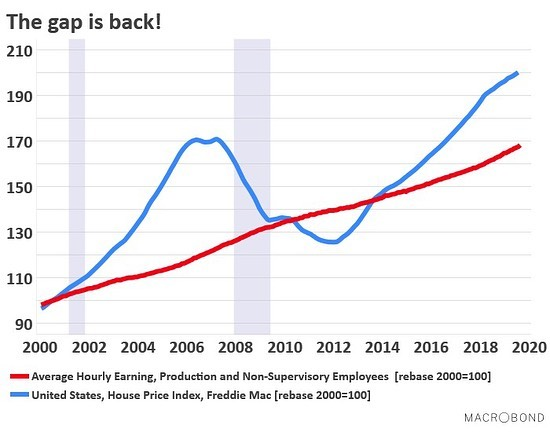
\includegraphics[height=8.5cm]{abb1}
\end{figure}

Dieser Graph wurde von Gabriel de Souza Tomitsuka mithilfe von Macrobond erstellt.
\newline

\textbf{Abbildung 2: Subprime-Kreditgeber}
\newline
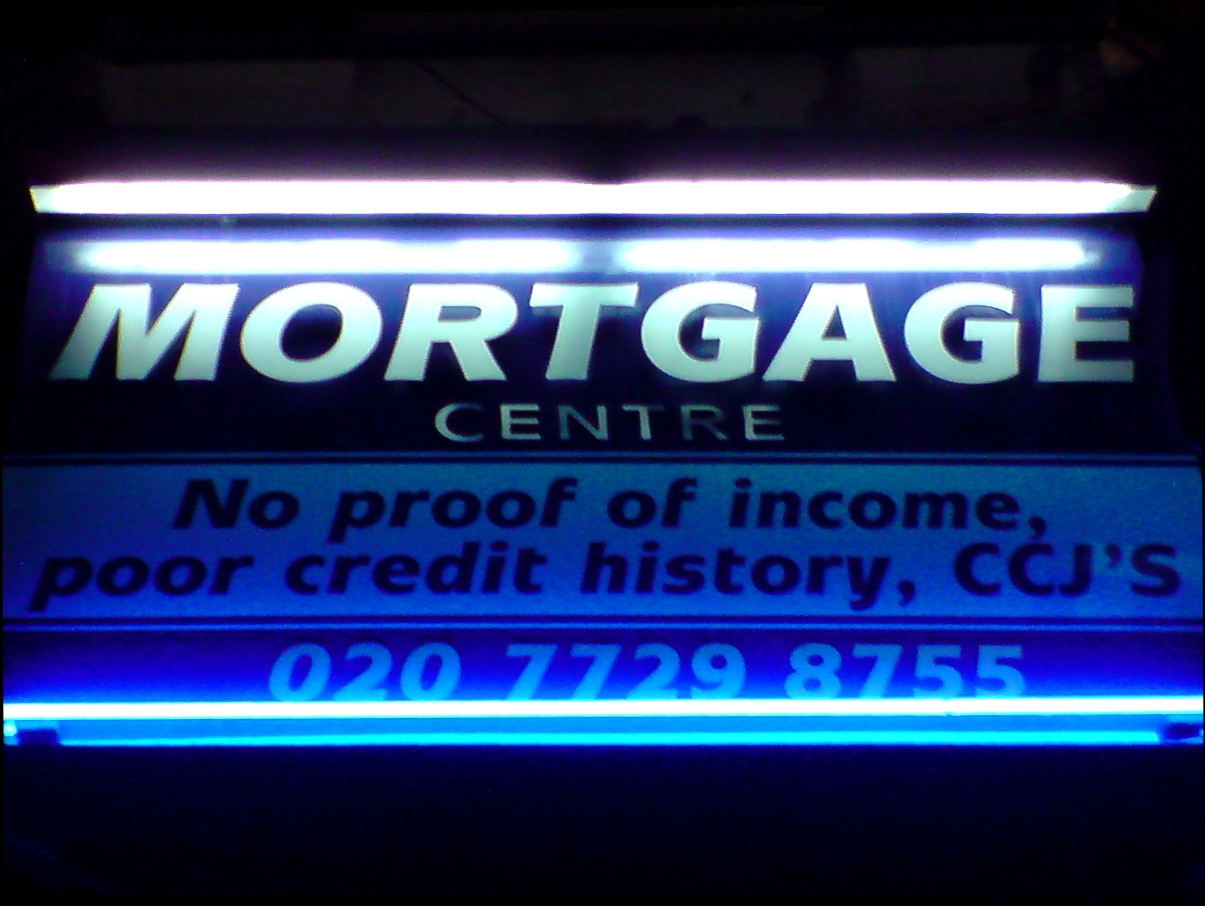
\includegraphics[height=8.5cm]{abb2}
\newpage
\textbf{Abbildung 3: Wachstum und Fall des HPIs}
\newline
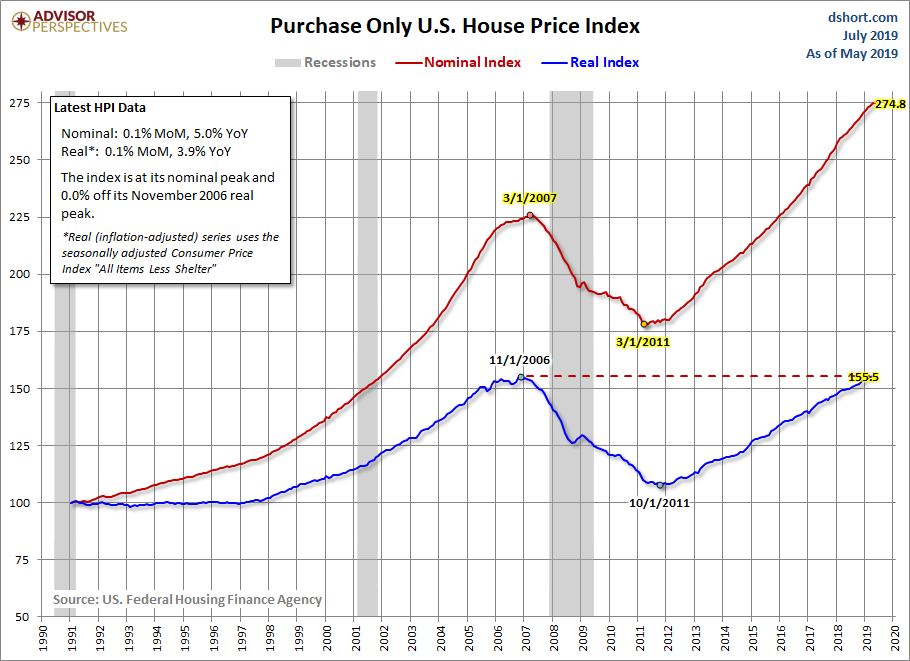
\includegraphics[width=\textwidth]{abb3}

\textbf{Abbildung 4: Preis unterschiedlicher Subprime Triple-A CDO-Tranchen, 2007-2008}
\newline
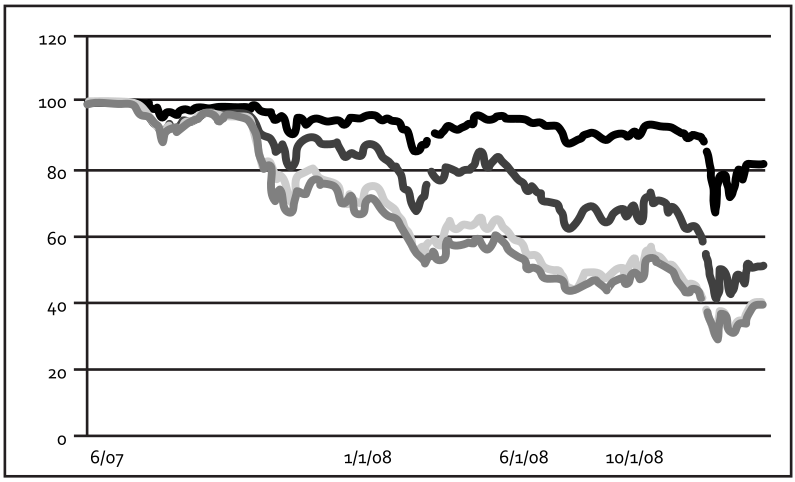
\includegraphics[width=\textwidth]{abb4}

\end{document}
http://web.mit.edu/rsi/www/pdfs/new-latex.pdf
http://web.mit.edu/rsi/www/pdfs/bibtex-format.pdf
http://www.ir.rochelleterman.com/sites/default/files/Helleiner%202011.pdf
Quelle 1: https://www.federalreserve.gov/econresdata/releases/mortoutstand/mortoutstand20090331.htm
Quelle 2: https://web.archive.org/web/20090419051155/http://www.sifma.org/uploadedFiles/Research/Statistics/SIFMA_USBondMarketOutstanding.pdf
Quelle 3: https://fraser.stlouisfed.org/timeline/financial-crisis
Quelle 4 (Doss, 2007): https://www.wsj.com/articles/SB116775515272364964
Quelle 5 (Creswell \& Bajaj, 2007): https://www.nytimes.com/2007/04/03/business/03lend.html
https://academic.oup.com/cje/article/33/4/563/1730705
GS: https://www.goldmansachs.com/insights/pages/learning-from-a-century-us-recessions/report.pdf
Buffett: https://www.youtube.com/watch?v=MQcPC31KRqA
Dimon: https://www.youtube.com/watch?v=QE3QwTA5ujE
Dimon text: https://www.jpmorganchase.com/corporate/investor-relations/document/annualreport-2018.pdf
EU: https://europa.eu/rapid/press-release_MEMO-08-123_en.htm?locale=en
ä \"a
ö \"o
ü \"u
ß
(28.09.19)
Ap. 1: mit Macro Bond selbst erstellt
Ap. 2: https://commons.wikimedia.org/wiki/File:P060708_22.03-02-retouched.jpg
Ap. 3: https://www.advisorperspectives.com/images/content_image/data/6c/6c77ccb14b1810a345ed768e3f8d5272.png